\documentclass{report}

\usepackage{amsmath, bm}
\usepackage[pdftex]{graphicx}
\usepackage{url}
\usepackage{float}

\def\bSig\mathbf{\Sigma}
\newcommand{\VS}{V\&S}
\newcommand{\tr}{\mbox{tr}}

\usepackage{caption}
\captionsetup[figure]{name=Web Figure}
\captionsetup[table]{name=Web Table}

\begin{document}

\title{Web Appendix for: Mixture models for distance sampling detection functions}

\author{David L. Miller, Len Thomas}

\maketitle

\section*{Outline}

This Web Appendix contains technical details of for the paper ``Mixture models for distance sampling detection functions'' by D. L. Miller and L. Thomas.

\section*{Web Appendix A - Optimization}
\label{s:optimization}

In practice, maximization is performed on the $\log$-likelihood. However, as noted in the literature (e.g. Gelman et al, 2004; Marin, Mengersen, Robert, 2005), mixture model likelihoods can be notoriously multimodal. This can cause problems when finding MLEs of the parameters. Here simulated annealing (SANN; Press et al., 1992, Chapter 10) was used to explore the parameter space (for 500 iterations) then after that the Broyden-Fletcher-Goldfarb-Shanno method (BFGS; Press et al., 1992, Chapter 10) was used to find the maxima (the implementations in the \textsf{R} function \texttt{optim()} were used). These two steps were run 5 times. This two step approach appears to be satisfactory in most cases. The EM algorithm (Dempster, Laird and Rubin, 1977) was tested although there was no significant performance increase (in terms of computational time or parameter precision) over using BFGS with SANN. To aid the optimization, analytic derivatives were also used; these are given in Web Appendix B.

\subsection*{Starting values}
Beavers and Ramsay (1998) give a method for estimating starting values for the scale parameter of a half-normal detection function. In the non-covariate case, the estimate is given as the intercept parameter from intercept only regression on $\log(y+\frac{w}{1000})$ (where $w$ denotes the truncation distance, as above). For covariate models, the equation used for the $\sigma$ is used in the regression and the estimated parameters from the linear regression are used as the starting values for the $\beta$s.

A similar approach can be use in the mixture case by dividing the sorted distances into $J$ equal parts. For each of these parts a Beavers and Ramsay-type estimate is used for the $\beta$s. The mixture weight $\phi_j$ had starting values of $1/J$ since there is no reason \textit{a priori} to believe anything else.

\subsection*{Parametrisation of the mixture proportions}

When using 2-point mixtures, the constraint that the mixture proportions must sum to unity is enforced by definition (since $\phi_2=1-\phi_1$). However, in $J$-point mixtures when $J>2$ ensuring that the proportions sum to 1 is not guaranteed. The obvious way to get around this would be to penalise the likelihood, should the optimisation procedure propose values for the $\phi_j$s that are not in accordance with this condition. This is, of course, inefficient and ugly. Instead, a parametrisation is used for the mixture proportions which yields $\phi_j$s that comply.

Rather than estimating the $\phi_j$s, estimate $\alpha_p$s ($p=1,\ldots,J$), where the relationship between the two is:
\begin{equation*}
\phi_j = F(\sum_{p=1}^j e^{\alpha_p}) - F(\sum_{p=1}^{j-1} e^{\alpha_p}) \qquad \text{for } 1\leq j \leq J-1
\end{equation*}
and
\begin{equation*}
\phi_J = 1-\sum_{j=1}^{J-1} \phi_j
\end{equation*}
where $F$ is any continuous CDF on $(0,\infty]$. Exponentiation ensures that $e^{\alpha_p}\geq0$, so $\alpha_p$ may lie anywhere on the real line, allowing unconstrained optimisation. Summing these orders the $\phi_j$s, since only offsets are estimated. Finally, using the cumulative density function ensures that the $\phi_j$s sum to $1$. In practise the $\text{Gamma}(3,2)$ CDF is (somewhat arbitrarily) used. Web Figure \ref{mmds-phifig} illustrates the relationship.

\begin{figure*}
\centering
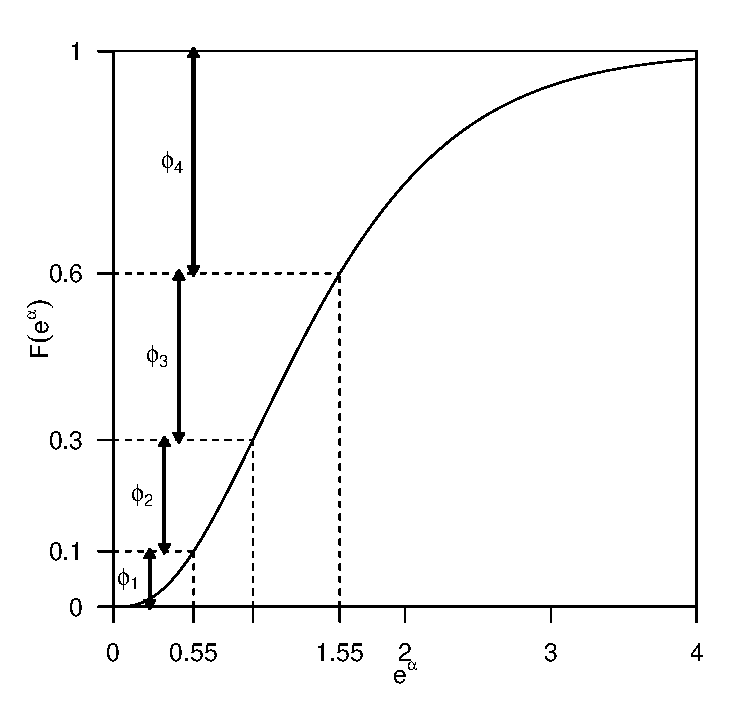
\includegraphics[width=0.5\textwidth]{figs/phidia.pdf}
\caption{The relationship between the mixture proportions, $\phi_j$ and the quantities estimated during the optimization procedure, $\alpha_p$.}
\label{mmds-phifig}
\end{figure*}

To transform from the $\phi_j$s back to the $\alpha_p$s we simply re-arrange the above expression.
\begin{equation*}
\alpha_p = \log_e \Big(F^{-1}\Big(\phi_j + F(\sum_{p=1}^{j-1} e^{\alpha_p})\Big) - \sum_{p=1}^{j-1} e^{\alpha_p}\Big).
\end{equation*}
Note that we only need as many $\alpha_p$s as we had $\phi_j$s, so we do not require any additional parameters.

\section*{Web Appendix B - Derivatives}

As mentioned above, maximization is performed on the $\log$-likelihood. In this section we give the derivations of the derivatives of the $\log$-likelihood, which were used to aid optimization. In the main paper we used the symbol $y$ to denote the distance from transect to object.  In practice, this distance is a perpendicular distance in the case of line transects and a radial distance for point transects.  Here, to avoid confusion, perpendicular distances in the line transect case are denoted by $x$ and radial distances in the point transect case are denoted by $r$.

\subsection*{Line transects}

Starting from the $\log$-likelihood:
\begin{equation}
l(\bm{\theta}, \bm{\phi}; \mathbf{x},\mathbf{Z}) = \sum_{i=1}^n \Big( \log \sum_{j=1}^J \phi_j g_j(x_i,\mathbf{Z}; \bm{\theta}_j) - \log \sum_{j=1}^J \phi_j \mu_{ij}\Big)
\label{lt-lik}
\end{equation}
we derive the derivatives with respect to the optimisation parameters.

\subsubsection*{With respect to $\beta_{0j*}$}

For the intercept terms (also considering in the non-covariate case, these are just the parameters), the parameters have no effect outside of their mixture (ie. $\beta_{0j*}$ only has an influence on mixture component $j*$), so we can write:
\begin{equation*}
\frac{\partial l(\bm{\theta},\bm{\phi}; \mathbf{x},\mathbf{Z})}{\partial \beta_{0j*}} = \sum_{i=1}^n \frac{1}{g(x_i,\mathbf{Z}; \bm{\theta},\bm{\phi})} \phi_{j*} \frac{\partial}{\partial \beta_{0j*}} g_{j*}(x_i,\mathbf{Z}; \bm{\theta}_{j*})  - \frac{\phi_{j*}}{\mu_i}  \frac{\partial}{\partial \beta_{0j*}} \mu_{ij*}.
\end{equation*}
Now, to first find $\frac{\partial}{\partial \beta_{0j*}} g_{j*}(x_i,\mathbf{Z}; \bm{\theta}_{j*})$:
\begin{equation*}
\frac{\partial g_{j*}(x_i,\mathbf{Z}; \bm{\theta}_{j*})}{\partial \beta_{0j*}} = \frac{\partial}{\partial \beta_{0j*}} \exp\Big( -\frac{x_i^2}{2\sigma_{j*}^2} \Big),
\end{equation*}
applying the chain rule and remembering that $\sigma_{j*}$ is a (trivial) function of the $\beta_{0j}$s:
\begin{equation*}
\frac{\partial g_{j*}(x_i,\mathbf{Z}; \bm{\theta}_{j*})}{\partial \beta_{0j*}} = \Big( \frac{x_i}{\sigma_{j*}}\Big)^2 \exp \Big(-\frac{x_i^2}{2 \sigma_{j*}^2}\Big)
\end{equation*}

Expressing $\mu_{ij*}$ in terms of the error function, $\text{Erf}$:
\begin{align}
\frac{\partial \mu_{ij*}}{\partial \beta_{0j*}} &= \frac{\partial}{\partial \beta_{0j*}} \Big( \sqrt{\frac{\pi}{2}} \sigma_{j*} \text{Erf}\Big(\frac{w}{\sqrt{2\sigma_{j*}^2}}\Big) \Big) \notag \\
&= \text{Erf}\Big(\frac{w}{\sqrt{2\sigma_{j*}^2}}\Big) \frac{\partial}{\partial \beta_{0j*}} \Big( \sqrt{\frac{\pi}{2}} \sigma_{j*} \Big) + \sqrt{\frac{\pi}{2}} \sigma_{j*} \frac{\partial}{\partial \beta_{0j*}} \Big(\text{Erf}\Big(\frac{w}{\sqrt{2\sigma_{j*}^2}}\Big) \Big)\label{app-mu-erf}
\end{align}
To find $\frac{\partial}{\partial \beta_{0j*}} \text{Erf}\Big(\frac{w}{\sqrt{2\sigma_{j*}^2}}\Big)$, note that we can write and then apply the chain rule:
\begin{align*}
\frac{\partial}{\partial \beta_{0j*}} \text{Erf}\Big(\frac{w}{\sqrt{2\sigma_{j*}^2}}\Big) &= \frac{\partial}{\partial \beta_{0j*}} S(u(\sigma_{j*}))\\
&= \frac{\partial S(u)}{\partial u} \frac{\partial u(\sigma_{j*})}{\partial \sigma_{j*} } \frac{\partial \sigma_{j*}}{\partial \beta_{0j*}}
\end{align*}
where 
\begin{align*}
S(u) = \int_0^{u} \exp(-t^2) \text{d}t \quad \text{and} \quad u(\sigma_{j*})=\frac{w}{\sqrt{2\sigma_{j*}^2}}.
\end{align*}
Their derivatives being
\begin{align*}
\frac{\partial S(u)}{\partial u} = \frac{2}{\sqrt{\pi}} \exp(-u^2) \text{,} \quad \frac{\partial u(\sigma_{j*})}{\partial \sigma_{j*}} = -\frac{w}{\sqrt{2}}\sigma_{j*}^{-2}.
\end{align*}
Given these terms, it is just a case of multiplying them:
\begin{align*}
\frac{\partial S(u)}{\partial u} \frac{\partial u(\sigma_{j*})}{\partial \sigma_{j*} } \frac{\partial \sigma_{j*}}{\partial \beta_{0j*}} = - \sqrt{\frac{2}{\pi}} \frac{w}{\sigma_{j*}} \exp\Big( -\frac{w^2}{2\sigma_{j*}^2} \Big)
\end{align*}
Substituting into (\ref{app-mu-erf}):
\begin{equation*}
\frac{\partial \mu_{ij*}}{\partial \beta_{0j*}} =  \mu_{ij*} - w \exp\Big( -\frac{w^2}{2\sigma_{j*}^2} \Big)
\end{equation*}
Finally, the derivative is:
\begin{equation*}
\frac{\partial l(\bm{\theta}, \bm{\phi}; \mathbf{x},\mathbf{Z})}{\partial \beta_{0j*}} = \sum_{i=1}^n \Big( \frac{x_i}{\sigma_{j*}}\Big)^2 \phi_{j*} \frac{g_{j*}(x_i,\mathbf{Z}; \bm{\theta}_{j*})}{g(x_i,\mathbf{Z}; \bm{\theta},\bm{\phi})}  - \frac{\phi_{j*}}{\mu_i} (\mu_{ij*} - w g_{j*}(w,\mathbf{Z}; \bm{\theta}_{j*})).
\end{equation*}


\subsection*{With respect to $\beta_{k*}$}

Derivatives with respect to the common covariate parameters are found in a similar way to above. The expressions are slightly more complicated since the $\beta_k$s effect all of the mixture components.
\begin{equation*}
\frac{\partial l(\bm{\theta},\bm{\phi}; \mathbf{x},\mathbf{Z})}{\partial \beta_{k*}} = \sum_{i=1}^n \Big( \frac{1}{g(x_i,\mathbf{Z}; \bm{\theta},\bm{\phi})} \sum_{j=1}^J \phi_j \frac{\partial}{\partial \beta_{k*}} g_j(x_i,\mathbf{Z}; \bm{\theta}_j) - \frac{1}{\mu_i} \sum_{j=1}^J \phi_j \frac{\partial}{\partial \beta_{k*}}\mu_{ij}\Big)
\end{equation*}
Every $\sigma_{j}$ is a function of the $\beta_{k}$s, so:
\begin{align*}
\frac{\partial \sigma_{j}}{\partial \beta_{k*}} &= \frac{\partial}{\partial \beta_{k*}} \exp \Big( \beta_{0j} + \sum_{k=1}^K z_{ik} \beta_{k}\Big),\\
&= z_{ik*}\sigma_{j}.
\end{align*}
Hence:
\begin{equation*}
 \frac{\partial}{\partial \beta_{k*}} \exp\Big( -\frac{x_i^2}{2\sigma_{j}^2} \Big) = z_{k*} \Big( \frac{x_i}{\sigma_{j}}\Big)^2 \exp \Big(-\frac{x_i^2}{2 \sigma_{j}^2}\Big) = z_{k*} \Big( \frac{x_i}{\sigma_{j}}\Big)^2 g_j(x_i,\mathbf{Z}; \bm{\theta}_j).
 \label{detfct-deriv-k}
\end{equation*}
And so for the $\mu_{ij}$s:
\begin{equation*}
\frac{\partial \mu_{ij}}{\partial \beta_{k*}} = z_{ik*} \Big( \mu_{ij} - w \exp\Big( -\frac{w^2}{2\sigma_{j}^2} \Big) \Big)
\end{equation*}
The derivative is then:
\begin{equation*}
\frac{\partial l(\bm{\theta},\bm{\phi}; \mathbf{x},\mathbf{Z})}{\partial \beta_{k*}} = \sum_{i=1}^n \Big( \frac{1}{g(x_i,\mathbf{Z}; \bm{\theta},\bm{\phi})} \sum_{j=1}^J \phi_j  z_{k*} \Big( \frac{x_i}{\sigma_{j}}\Big)^2 g_j(x_i,\mathbf{Z}; \bm{\theta}_j) - \frac{1}{\mu_i} \sum_{j=1}^J \phi_j z_{ik*} ( \mu_{ij} - w g_j(x_i,\mathbf{Z}; \bm{\theta}_j) )\Big)
\end{equation*}

\subsubsection*{With respect to $\alpha_{j*}$}

First note that we can write the likelihood (\ref{lt-lik}) as:
\begin{align*}
l(\bm{\theta},\bm{\phi}; \mathbf{x},\mathbf{Z}) = \sum_{i=1}^n\Big( &\log \Big( \sum_{j=1}^{J-1} \phi_j g_j(x_i,\mathbf{Z}; \bm{\theta}_j) + (1-\sum_{j=1}^{J-1} \phi_j) g_J(x_i,\mathbf{Z}; \bm{\theta}_J)\Big) \\
&-  \log \Big(\sum_{j=1}^{J-1} \phi_j \mu_{ij} + (1-\sum_{j=1}^{J-1} \phi_j) \mu_{ij} \Big) \Big)
\end{align*}
The derivatives with respect to the $\alpha_{j*}$ of this expression are then:
\begin{align}
\frac{\partial l(\bm{\theta},\bm{\phi}; \mathbf{x},\mathbf{Z})}{\partial \alpha_{j*}} = &\Big( \sum_{i=1}^n \frac{1}{g(x_i,\mathbf{Z}; \bm{\theta},\bm{\phi})} \Big( \sum_{j=1}^{J-1} g_j(x_i,\mathbf{Z}; \bm{\theta}_j) \frac{\partial \phi_j}{\partial \alpha_{j*}}  -g_J(x_i,\mathbf{Z}; \bm{\theta}_J) \sum_{j=1}^{J-1}  \frac{\partial \phi_j}{\partial \alpha_{j*}}\Big) \notag \\
&- \frac{1}{\mu_i} \Big(\sum_{j=1}^{J-1} \mu_{ij} \frac{\partial \phi_j}{\partial \alpha_{j*}} - \mu_{iJ} \sum_{j=1}^{J-1}   \frac{\partial \phi_j}{\partial \alpha_{j*}} \Big)\Big) \label{app-lik-alphad}
\end{align}
Finding the derivatives is then simply a matter of finding the derivatives of $\phi_{j}$ with respect to $\alpha_{j*}$ and substituting them back into (\ref{app-lik-alphad}).
\begin{equation*}
\frac{\partial \phi_j}{\partial \alpha_{j*}} = \frac{\partial}{\partial \alpha_{j*}}F(\sum_{p=1}^j e^{\alpha_p}) - \frac{\partial}{\partial \alpha_{j*}} F(\sum_{p=1}^{j-1} e^{\alpha_p}).
\end{equation*}
Looking at each of the terms:
\begin{equation*}
\frac{\partial}{\partial \alpha_{j*}} F(\sum_{p=1}^j e^{\alpha_p})=A_{j}=\begin{cases}
e^{\alpha_{j*}}f(\sum_{p=1}^j e^{\alpha_p})& \text{for $j\geq j*$},\\
0 & \text{for $j<j*$}.
\end{cases}
\end{equation*}
and
\begin{equation*}
\frac{\partial}{\partial \alpha_{j*}} F(\sum_{p=1}^{j-1} e^{\alpha_p})=A_{(j-1)}=\begin{cases}
e^{\alpha_{j*}}f(\sum_{p=1}^{j-1} e^{\alpha_p})& \text{for $j-1\geq j*$},\\
0 & \text{for $j-1<j*$}.
\end{cases}
\end{equation*}
So
\begin{equation*}
\frac{\partial \phi_j}{\partial \alpha_{j*}} = A_j - A_{j-1}.
\end{equation*}
Substituting these back into (\ref{app-lik-alphad}) and re-arranging gives:
\begin{align*}
\frac{\partial l(\bm{\theta},\bm{\phi}; \mathbf{x},\mathbf{Z})}{\partial \alpha_{j*}} = \sum_{i=1}^n & \Big( \frac{1}{g(x_i,\mathbf{Z}; \bm{\theta},\bm{\phi})} \sum_{j=1}^{J-1} (A_j - A_{j-1}) (g_j(x,\mathbf{Z}; \bm{\theta}_j) - g_J(x,\mathbf{Z}; \bm{\theta}_J))\\
&- \frac{1}{\mu_i} \sum_{j=1}^{J-1}(A_j - A_{j-1})(\mu_{ij} - \mu_{iJ}) \Big)
\end{align*}

\subsection*{Point transects}

We now provide the corresponding quantities for point transects, starting from the $\log$-likelihood:
\begin{equation}
l(\bm{\theta}, \bm{\phi}; \mathbf{r},\mathbf{Z}) = n \log 2 \pi + \sum_{i=1}^n \Big( \log r_i + \log \sum_{j=1}^J \phi_j g_j(r_i,\mathbf{Z}; \bm{\theta}_j) - \log \sum_{j=1}^J \phi_j \nu_{ij}\Big).
\label{pt-lik}
\end{equation}


\subsubsection*{With respect to $\beta_{0j}$}

From (\ref{pt-lik}), one can see that we obtain:
\begin{align*}
\frac{\partial l(\bm{\theta}, \bm{\phi}; \mathbf{r},\mathbf{Z})}{\partial \beta_{0j*}}  &= \sum_{i=1}^n \Big( \frac{\partial}{\partial \beta_{0j*}} \log \sum_{j=1}^J \phi_j g_j(r_i,\mathbf{Z}; \bm{\theta}_j) - \frac{\partial}{\partial \beta_{0j*}}\log \sum_{j=1}^J \phi_j \nu_{ij}\Big)\\
&= \sum_{i=1}^n \Big( \frac{ \phi_{j*} \frac{\partial}{\partial \beta_{0j*}}  g_{j*} (r_i,\mathbf{Z}; \bm{\theta}_j)}{g(r_i,\mathbf{Z}; \bm{\theta}, \bm{\phi})} - \frac{ \phi_{j*}\frac{\partial}{\partial \beta_{0j*}}  \nu_{ij*} }{ \sum_{j=1}^J \phi_j \nu_{ij}}\Big)
\end{align*}
the first part of which (the derivatives of the detection function) are as in the line transect case. The derivatives of $\nu_{ij}$ are simpler in the point transect case, since there is an easy analytic expression for $\nu_{ij}$ when $g_j$ is half-normal :
\begin{equation*}
\nu_{ij} = 2 \pi \sigma_{ij}^2 (1-\exp (-w^2/2\sigma_{ij}^2 ))
\end{equation*}
then simply applying the product rule yields:
\begin{equation*}
\frac{\partial \nu_{ij}}{\partial \beta_{0j*}} = 2 (\nu_{ij*} + \pi w^2 g_{j*}(w)).
\end{equation*}
Substituting this into the above expression:
\begin{equation*}
\frac{\partial l(\bm{\theta}, \bm{\phi}; \mathbf{r},\mathbf{Z})}{\partial \beta_{0j*}}  = \sum_{i=1}^n \Big( \frac{ \phi_{j*} (r_i/\sigma_{j*})^2 g_{j*}(r_i,\mathbf{Z}; \bm{\theta}_{j*})}{g(r_i,\mathbf{Z}; \bm{\theta}, \bm{\phi})} - \frac{ \phi_{j*} 2 (\nu_{j*} + \pi w g_{j*}(w)) }{ \sum_{j=1}^J \phi_j \nu_{ij}}\Big)
\end{equation*}

\subsubsection*{With respect to $\beta_{k*}$}

Again working from (\ref{pt-lik}), we obtain:
\begin{align*}
\frac{\partial l(\bm{\theta}, \bm{\phi}; \mathbf{r},\mathbf{Z})}{\partial \beta_{k*}}  &= \sum_{i=1}^n \Big( \frac{\partial}{\partial \beta_{k*}} \log \sum_{j=1}^J \phi_j g_j(r_i,\mathbf{Z}; \bm{\theta}_j) - \frac{\partial}{\partial \beta_{k*}}\log \sum_{j=1}^J \phi_j \nu_{ij}\Big)\\
&= \sum_{i=1}^n \Big( \frac{ \sum_{j=1}^J \phi_{j} \frac{\partial}{\partial \beta_{k*}}  g_{j} (r_i,\mathbf{Z}; \bm{\theta}_j)}{g(r_i,\mathbf{Z}; \bm{\theta}, \bm{\phi})} - \frac{ \sum_{j=1}^J \phi_{j}\frac{\partial}{\partial \beta_{k*}}  \nu_{ij} }{ \sum_{j=1}^J \phi_j \nu_{ij}}\Big)
\end{align*}
The derivatives of $g_j$ are as in (\ref{detfct-deriv-k}). For $\nu_{ij}$:
\begin{equation*}
\frac{\partial \nu_{ij}}{\partial \beta_{k*}} =  2z_{ik*}(\nu_{ij} - \pi w^2 g_j(w))
\end{equation*}
Putting that together:
\begin{equation*}
\frac{\partial l(\bm{\theta}, \bm{\phi}; \mathbf{r},\mathbf{Z})}{\partial \beta_{k*}}  = \sum_{i=1}^n \Big( \frac{ \sum_{j=1}^J \phi_{j} z_{k*} \Big( \frac{x_i}{\sigma_{j}}\Big)^2 g_j(x_i,\mathbf{Z}; \bm{\theta}_j)}{g(r_i,\mathbf{Z}; \bm{\theta}, \bm{\phi})} - \frac{ \sum_{j=1}^J \phi_{j}2z_{ik*}(\nu_{ij} - \pi w^2 g_j(w)) }{ \sum_{j=1}^J \phi_j \nu_{ij}}\Big)
\end{equation*}


\section*{Web Appendix C - Variance estimation}

Variances of both $\hat{N}$ and $\hat{P}_a$ can be estimated for both non-covariate models and covariate models using standard methods (Borchers, Buckland and Zucchini, 2002, Appendix C; Marques and Buckland, 2004, Section 3.3.3; Borchers et al, 1998).

In the most general case, the variance of $\hat{N}$ is estimated by:
\begin{equation*}
\hat{\text{Var}}\left( \hat{N} \right) = \left(\frac{\partial \hat{N}}{\partial\hat{\bm{\Theta}}}\right)^\text{T}\hat{\mathbf{I}}(\hat{\bm{\Theta}})^{-1}\frac{\partial \hat{N}}{\partial\hat{\bm{\Theta}}} + \sum_{i=1}^n \frac{(1-p_i)}{p_i^2}
\end{equation*}
where $\hat{\mathbf{I}}(\hat{\bm{\Theta}})^{-1}$ is the inverse of the Fisher information matrix,  $\hat{\bm{\Theta}}$ is a vector of all of the maximum likelihood estimates of the parameters of the detection function ($\hat{\bm{\Theta}}=(\hat{\bm{\theta}},\hat{\bm{\phi}})$) and all other notation is as in previous sections.

Then for the average detectability:
\begin{align*}
\hat{\text{Var}}\left( \hat{P}_a \right) = \hat{P}_a^2\left\{ \vphantom{\frac{\frac{a}{b}^b}{b}} \frac{\hat{\text{Var}}(\hat{N})}{\hat{N}^2}\right. &+\left.\frac{\left(\frac{\partial \hat{P}_a}{\partial\bm{\hat{\Theta}}}\right)^\text{T}\hat{\mathbf{I}}(\hat{\bm{\Theta}})^{-1}\frac{\partial \hat{P}_a}{\partial\bm{\hat{\Theta}}}+\sum_{i=1}^n (1-p_i)}{n^2} \right. \\
 & \left. - \frac{2\left(\left(\frac{\partial \hat{N}}{\partial\bm{\hat{\Theta}}}\right)^\text{T}\hat{\mathbf{I}}(\hat{\bm{\Theta}})^{-1}\frac{\partial \hat{P}_a}{\partial\bm{\hat{\Theta}}}+\sum_{i=1}^n\frac{(1-p_i)}{p_i^2}\right)}{n\hat{N}}\right\}.\\
\end{align*}

\section*{Web Appendix D - Simulation parameters}

The formulation used for the exponential power series (EPS) detection function in simulation E1 was:
\begin{equation*}
g(y,\mathbf{z}; \lambda, b_1) =  \exp(-(y/\lambda)^{-b_1})),
\end{equation*}
which has the following pdf:
\begin{equation*}
f(y,\mathbf{z}; \lambda, b_1) =  \frac{\exp(-(y/\lambda)^{-b_1})),}{\lambda\Gamma(1+\frac{1}{b_1})}
\end{equation*}
where $\lambda=\exp(\beta_1)$ is a scale parameter and $b_1$ is a \textit{shape parameter}.

The formulation for the hazard-rate mixture in simulation E2 was:
\begin{equation*}
g(y,\mathbf{z}; \bm{\theta}, \bm{\phi}) = \sum_{j=1}^J \phi_j (1-\exp(-(y/\sigma_j)^{-b_j})),
\end{equation*}
where $b_j$ is the shape parameter associated with the $j^\text{th}$ mixture component.

\begin{table}[htbp]
\centering
\caption{Parameters of the detection functions used in the simulations in Section 3 and the true average detection probability ($P_a$) for each model. Note that for covariate models, $\beta_1$ corresponds to the intercept of the first mixture component, $\beta_2$ to the intercept of the second mixture component and $\beta_3$ to the coefficient for the (common) covariate effect. Numbering is as in Figures 2 and 3 in the main article.}
\begin{tabular}{c c c c c c c c c c}\\
\hline
\hline
Model & Scenario & $\beta_1$ & $\beta_2$ & $\beta_3$ & $\pi_1$ & $\pi_2$ & $b_1$ & $b_2$ & $P_a$ \\
\hline
\hline
Line transect & A1 & -0.223 & -1.897 & &  0.3 & & & & 0.369\\
 & A2 & -0.511 & -2.303 & &  0.7 & & & & 0.514\\
 & A3 &  2.303 & -1.609 & & 0.15 & & & & 0.363\\
 & A4 & -0.357 & -2.996 & &  0.6 & & & & 0.471\\
Point transect &B1 & -0.223 & -1.897 & &  0.3 & & & & 0.24\\
 & B2 & -0.511 & -2.303 & &  0.7 & & & & 0.384\\
 & B3 &  2.303 & -1.609 & & 0.15 & & & & 0.218\\
 & B4 & -0.357 & -2.996 & &  0.6 & & & & 0.378\\
3-point & C1 &  -0.22 &  -0.69 &  -2.3 & 0.3 & 0.3 & & & 0.505\\
 & C2 &   2.71 &  -1.39 &  -3.0 & 0.1 & 0.4 & & & 0.257\\
Covariate & D1 & -2.303 & -0.288 & -0.511 & 0.4 & & & & 0.422\\
 & D2 & -1.609 & -0.223 & -0.916 & 0.4 & & & & 0.389\\
 EPS & E1 & -0.534 & & & & & 1.5& & 0.5 \\
 Hazard-rate & E2 & -1.69 & -0.304 & & 0.5 & & 7 & 7 & 0.5\\
\hline
\end{tabular}
\label{partable}
\bigskip
\end{table}



\section*{Web Appendix E - Simulation results}

Figure 3 in the main paper gives boxplots showing the distribution of estimated probability of detection, $P_a$ obtained if only the mixture models are included in the candidate model set.  Here, we show the the distribution of estimates when only K+A models are used (Web Figure \ref{sim-boxplots-cds}), the distribution of estimates when both mixture and K+A models are included (Web Figure \ref{sim-boxplots-combined}), and the proportion of time each model is chosen using the combined modelling strategy (Web Figure \ref{sim-barplot}).

\begin{figure}[H]
\centering
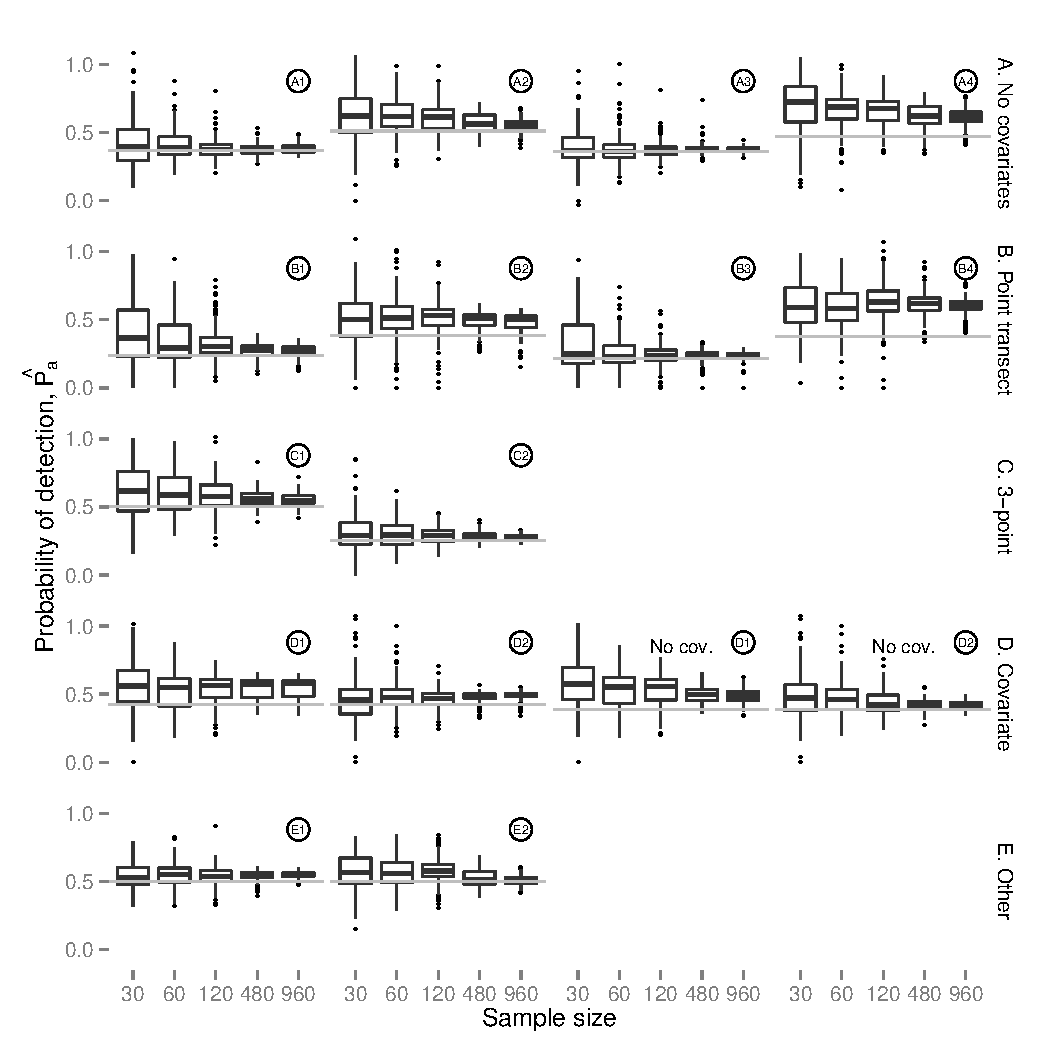
\includegraphics[width=\textwidth]{simulations/pa-plot-cds.pdf}
\caption{Simulation results: boxplots of the estimated average detection probabilities, $P_a$, for the best K+A model (by AIC score). Grey lines indicate the true value of the average detection probability.}
\label{sim-boxplots-cds}
\end{figure}

\begin{figure}[H]
\centering
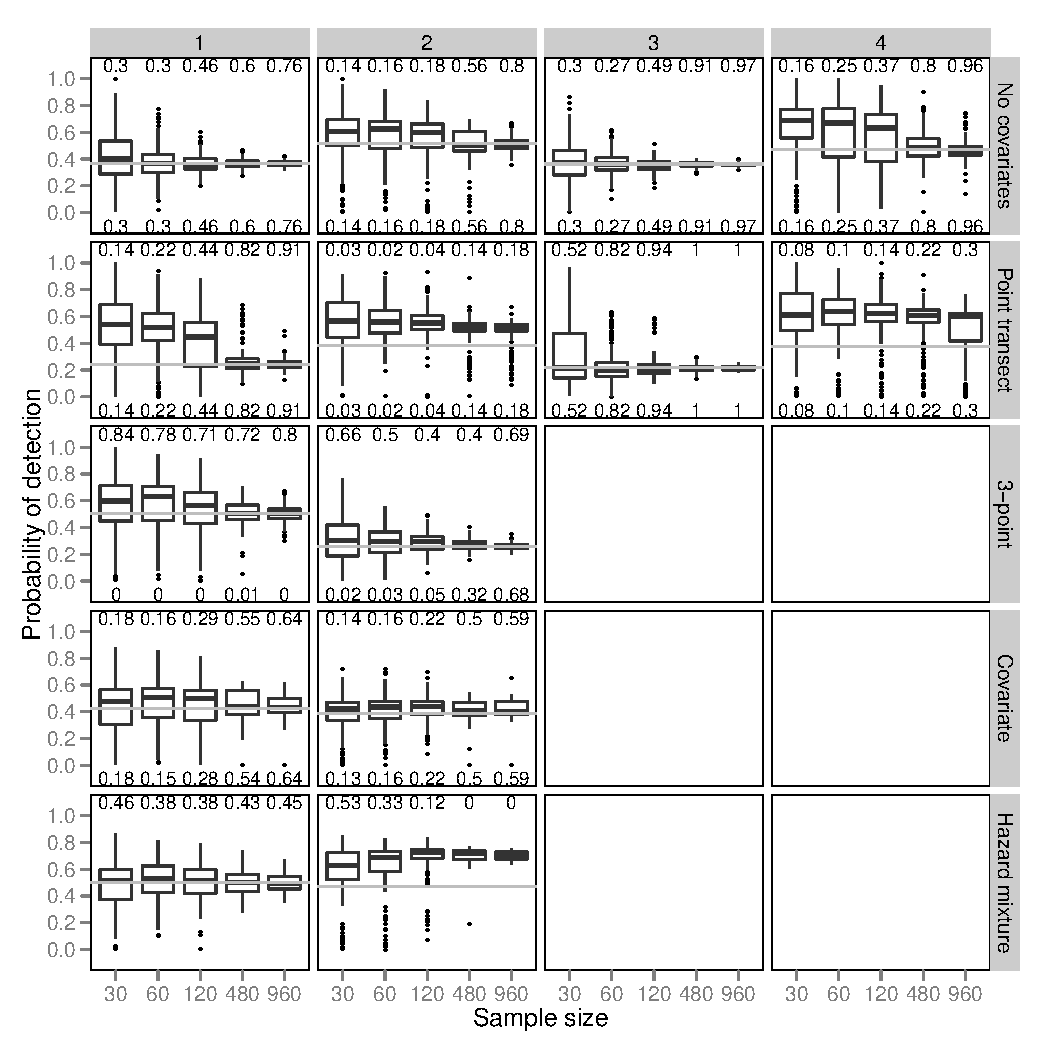
\includegraphics[width=\textwidth]{simulations/pa-plot-combined.pdf}
\caption{Simulation results: boxplots of the estimated average detection probabilities, $P_a$, for the best model (by AIC score) for both mixture and K+A models. In each case the best overall model was selected, reflecting the modelling approach undertaken in practice. Grey lines indicate the true value of the average detection probability. Numbers underneath each boxplot give the proportion of AIC best models that were of the same form as the model that the data was simulated from (e.g., in scenario D1, the proportion of AIC best models that were 2-point mixtures that included the covariate in the model). Numbers above each model give the proportion of times that the AIC best model was a 2- or 3-point mixture model.}
\label{sim-boxplots-combined}
\end{figure}

\begin{figure}[H]
\centering
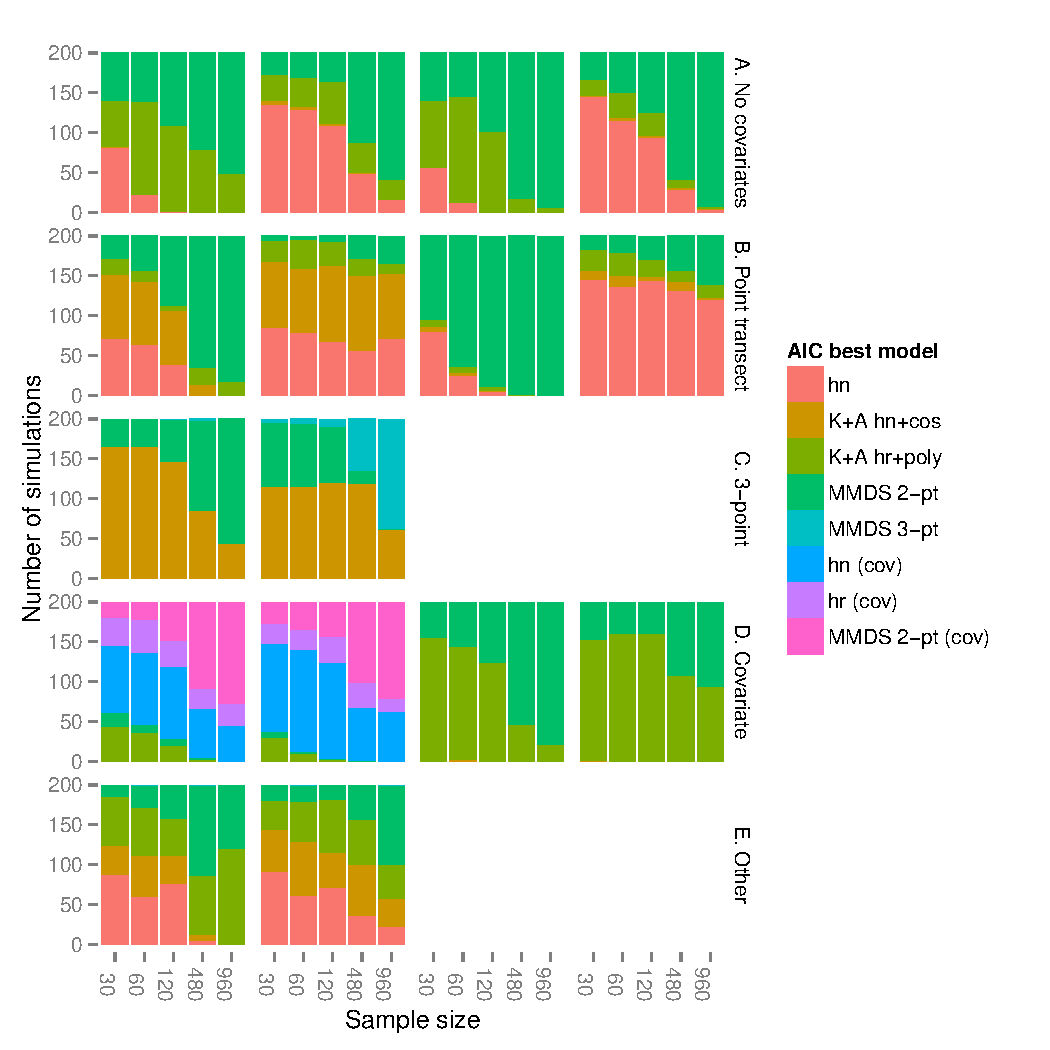
\includegraphics[width=\textwidth]{simulations/bar-winners.pdf}
\caption{Simulation results: stacked bar charts showing the number of models selected by AIC that fall into the given model classes. Layout is as in Web Figure 3, above. ``hn'' is a half-normal detection function and ``hr'' is a hazard-rate detection function (no adjustments/1-point mixture). K+A indicates a key function plus adjustment term model where ``cos'' is cosine and ``poly'' are simple polynomial adjustments. MMDS is a mixture model with 2 or 3 components (``2-pt'' or ``3-pt'', respectively). ``(cov)'' indicates that covariates were included in the model (no adjustments were allowed when covariates were used).}
\label{sim-barplot}
\end{figure}


\newpage
\section*{Web Appendix F - Case studies}

Before analysing the wood ant and amakihi data the variables nest size (for ants) and minutes after sunrise (for amakihi) were standardised by dividing the variable by its standard error. 

Plots of the best mixture detection function for the wood ant case study are given in Web Figure \ref{ants-nesthab} and for the amakihi in Web Figure \ref{amakihi}.

\begin{figure}[H]
\centering
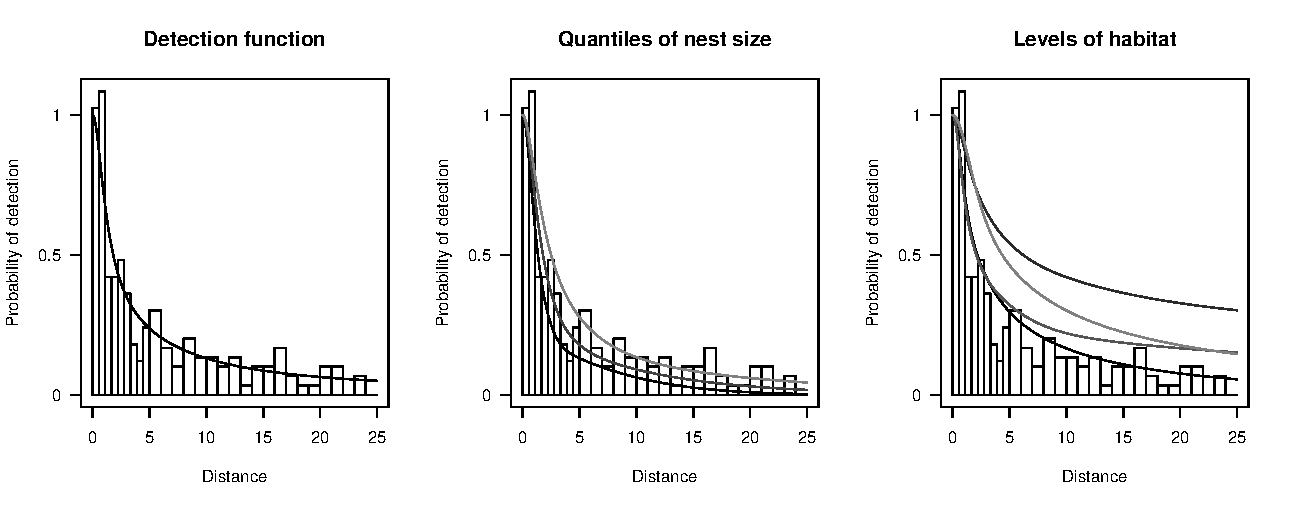
\includegraphics[width=0.3333\textwidth, trim=0 0 5.73228347in 0, clip=true]{analyses/ants-nesthab-1.pdf}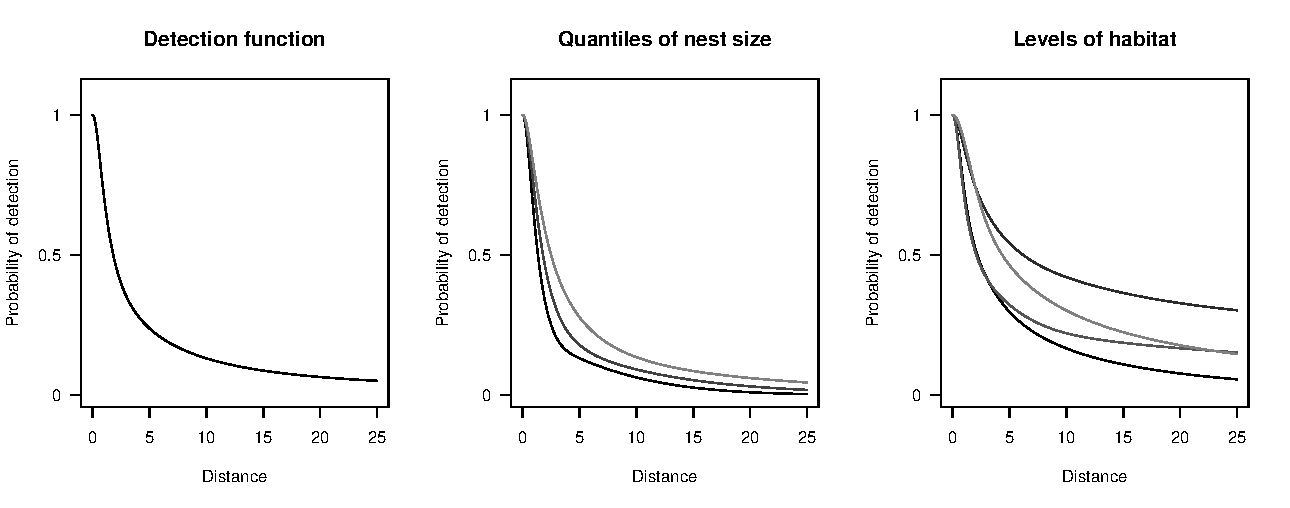
\includegraphics[width=0.6666\textwidth, trim=2.86614173in 0 0 0, clip=true]{analyses/ants-nesthab-2.pdf}
\caption{Plot of the detection functions for the AIC best model for the ants data set (2-point mixture with nest size and habitat as covariates). The first panel shows the average detection function (dashed lines are the two mixture components of the detection function, averaged over covariate values). The second and third panels show the quartiles of nest size and the levels of habitat type respectively.}
\label{ants-nesthab}
\end{figure}

\begin{figure}[H]
\centering
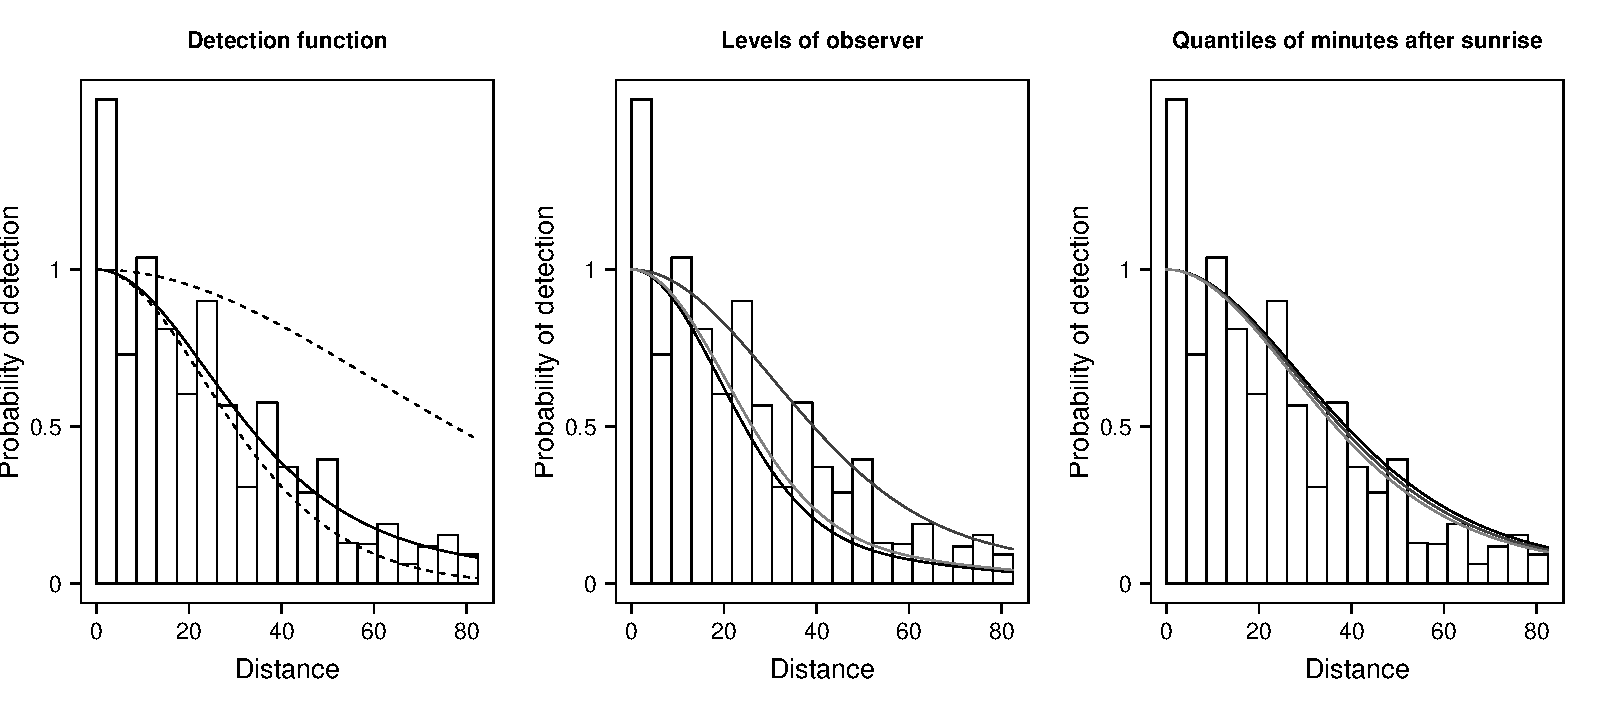
\includegraphics[width=0.3333\textwidth, trim=0 0 7.133334in 0, clip=true]{analyses/amakihi-om.pdf}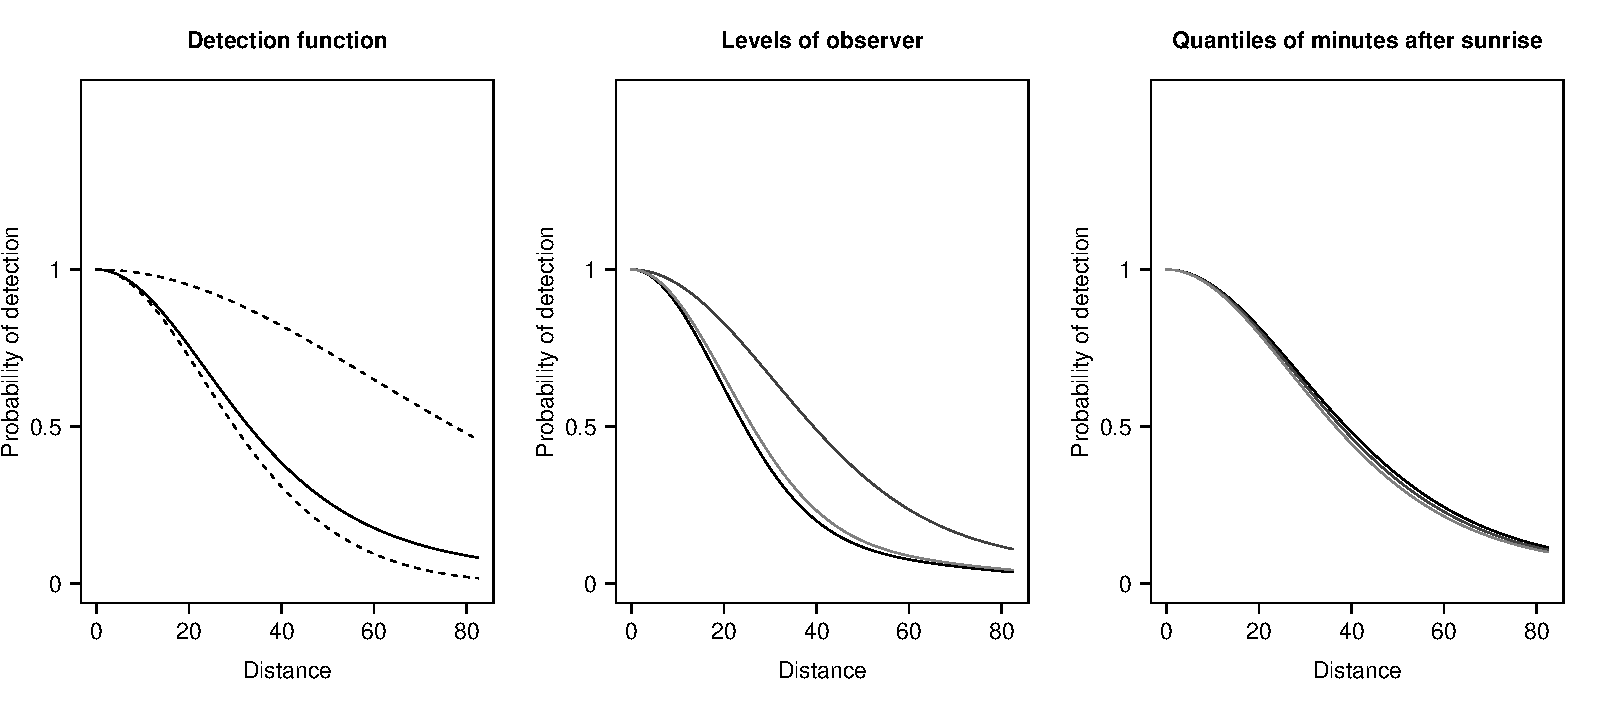
\includegraphics[width=0.6666\textwidth, trim=3.566667in 0 0 0, clip=true]{analyses/amakihi-om-hh.pdf}\\
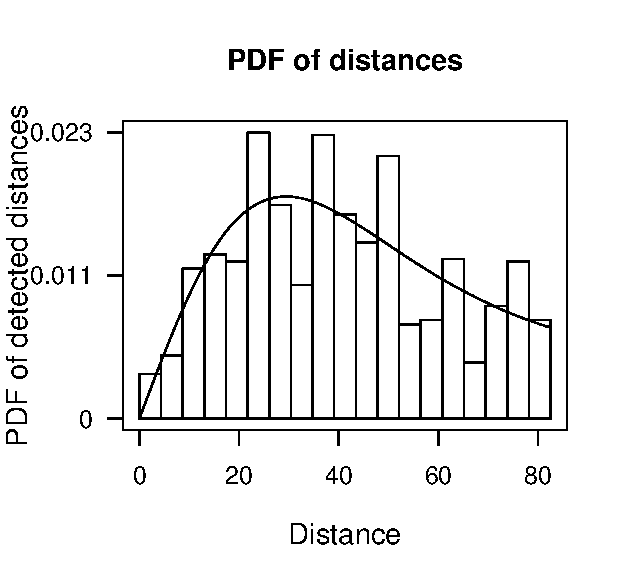
\includegraphics[width=0.4\textwidth]{analyses/amakihi-om-pdf.pdf}
\caption{Plots of the (AIC) best mixture model for the Amakihi data: a 2-point mixture with observer and minutes after sunrise as covariates. Top row: detection function averaged over covariates (dashed lines are each mixture component averaged over covariates), marginal detection function showing the levels of observer (averaged over the values of minutes after sunrise) and marginal detection function for minutes after sunrise ranging between 0 and 300 minutes (averaged over the levels of observer), as in Marques et al (2007). Bottom row: pdf of distances averaged over the covariate values.}
\label{amakihi}
\end{figure}






\begin{thebibliography}{}

\bibitem{ } Beavers, S. C., and Ramsey, F. L. (1998). Detectability analysis in transect surveys. \textit{Journal of Wildlife Management} \textbf{62}(3), pp. 948--957.

\bibitem{} Borchers, D. L., and Buckland, S. T. and Zucchini, W. (2002). \textit{Estimating animal abundance: closed populations}. Springer.

\bibitem{ }  Buckland, S. T., Anderson, D. R., Burnham, K. P., Laake, J. L., Borchers, D. L., and Thomas, L.  (2001). \textit{Distance sampling}. Oxford University Press. Oxford, UK.

\bibitem{ } Dempster, A.P., Laird,  N. M. and Rubin, D. B. (1977). Maximum likelihood from incomplete data via the EM algorithm. \textit{Journal of the Royal Statistical Society: Series B (Methodological)} \textbf{39}(1), 1--38.

\bibitem{ }  Gelman, A., Carlin, J. B., Stern, H. S., and Rubin, D. B. (2004). \textit{Bayesian data analysis}. CRC Press.

\bibitem{} Borchers, D. L., Buckland, S. T., Goedhart, P. W., Clarke, E. D. and Hedley, S. L. (1998). Horvitz-Thompson estimators for double-platform line transect surveys. \textit{Biometrics} \textbf{54}(4), 1221--1237.

\bibitem{ } Marin, J. M., Mengersen, K. and Robert, C. P. (2005). Bayesian modelling and inference on mixtures of distributions. \textit{Handbook of Statistics 25} D. Dey and C.R. Rao (eds). Elsevier-Sciences.

\bibitem{ } Marques, F. F. C. and Buckland, S. T. (2004). Covariate models for the detection function. In \textit{Advanced Distance Sampling}, pp. 31--47. S. T. Buckland, D. R. Anderson, K. P. Burnham, J. L. Laake, D. L. Borchers and L. Thomas (eds). Oxford University Press, Oxford.

\bibitem{ } Marques, T.A.,Thomas, L., Fancy, S.G., and Buckland, S.T. (2007) Improving Estimates of Bird Density Using Multiple-Covariate Distance Sampling. \textit{The Auk} \textbf{124},(4), 1229--1243.

\bibitem{ } Press, W. H., Teukolsky, S. A., Vetterling, W. T., Flannery, B. P. (1992). \textit{Numerical recipes: the art of scientific computing}. Cambridge University Press. 

\end{thebibliography}

\end{document}